%!TEX root = ../../../thesis.tex

Details of components in the electrode-electrolyte interface model and methods of determining its parameters have now been discussed.
Now come the measurements and fitting of the model parameters to the collected data.
Model parameters are first determined for various concentrations of phosphate buffered saline (PBS), then for comparison -- in a living sheep's spinal cavity.
This tells us whether a one-tenth concentration of PBS is in-fact a good substitute for cerebrospinal fluid (CSF), which it is assumed to be by implant engineers.


\section{Phosphate Buffered Saline}
    Scott \& Single fitted parameters of their model to a one-tenth concentration (0.1X) of a standard solution of PBS \cite{Scott2014}.
    I measure and fit parameters not only to the one-tenth concentration of PBS but to a range of concentrations from 0.025X up to 1X.
    For the parameters that vary with PBS concentration, a fit of the parameter's value to concentration using regression analysis is made.
    Doing this gives a a model that can be used to predict the impedance response of an electrode array in a wide range of solution concentrations.

    Each of the PBS measurements were made in \SI{1}{\litre} glass bottles containing \SI{700}{\milli\litre} of PBS solution in each case.
    Measurements were made in a temperature environment that was set to \SI{23}{\degree} Celsius.
    All measurements were automated by the use of Python on a workstation running Linux that communicates with the measurement instruments and collects data.
    Each measurement set was repeated for each of the six concentrations of PBS used.
    The six concentrations of PBS measured are 0.025X, 0.05X, 0.1X, 0.25X 0.5X, and 1.0X the concentration of the standard stock solution.

    \subsection{Resistor Mesh}

      \begin{figure}
        \centering
        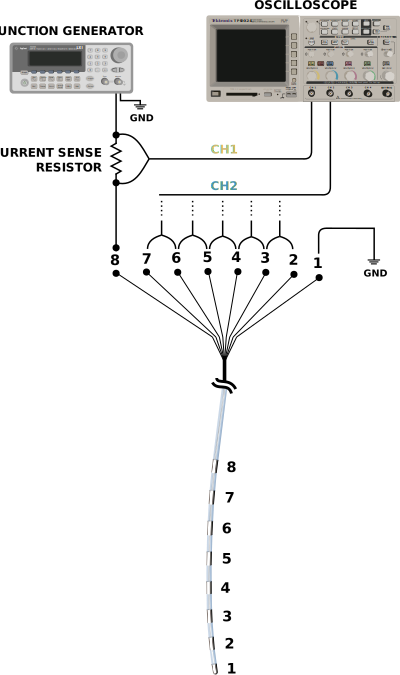
\includegraphics{content/pt2/08-InterfaceParameters/graphics/measurement_resistorMesh}
        \caption{\label{fig:pt2-measurement_resistorMesh}Illustration of measurement configuration used to to measure the electrode transimpedances. Each of the electrode pairs were measured one-after-the-other.}
      \end{figure}

      % TODO: Redraw the above diagram so as to be more compact

      With the elecrode immersed in a solutino of PBS a \SI{10}{\kilo\hertz} sinusoidal current having an amplitude of \SI{500}{\micro\ampere} was passed through the stimulus electrodes using an Agilent 33220A function generator.
      A current sense resistor was inserted in series with the stimulus electrodes.
      The differential voltage across a pair of non-stimulating electrodes and the voltage across the current sense resistor was measured using a Tektronix TPS 2024 oscilloscope.
      \Cref{fig:pt2-measurement_resistorMesh} shows the measurement configuration used when electrodes one and eight are used as the stimulus electrodes.

      \begin{figure}
        \centering
        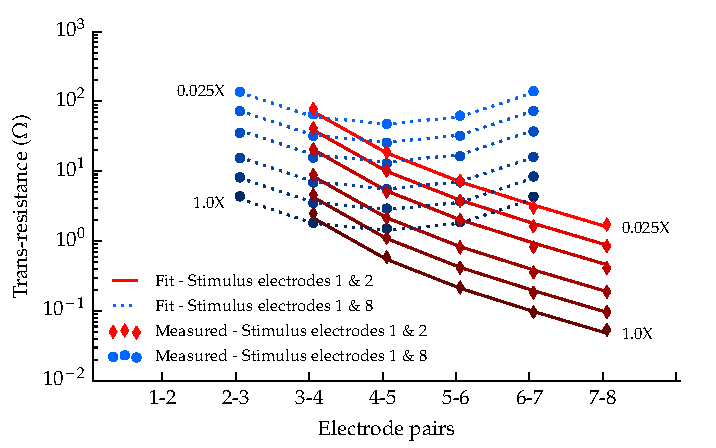
\includegraphics{content/pt2/07-InterfaceModel/graphics/graph_transimpedance_pbs}
        \caption{\label{fig:pt2-graph_transimpedance_pbs}Measured and fitted values of trans-impedance for both measurement configurations. Voltage measurements are made between adjacent pairs of electrodes as current is pushed through the stimulus electrodes.}
      \end{figure}

    \subsection{Series Resistance And Constant Phase Element}
        Discuss equipment and settings used to make the measurements.



        \Cref{fig:pt2-graph_transimpedance_pbs} shows measurement results for each pair of non-stimulated pair of electrodes along with simulated results using the fitted parameters.


        \begin{table}
          \centering
          \begin{tabular}{r | l}
            Parameter & Value \\
            \hline
            $R_{eri}$ ($\Omega$)& 0.407 / $\sigma$\\
            $R_{sri}$ ($\Omega$)& $R_{eri}\cdot 3/4$\\
            $R_{li}$ ($\Omega$)& 3.71 / $\sigma$ \\
            Depth (layers) & 5 \\
            Padding (layers) & 3 \\
          \end{tabular}
          \caption{\label{tab:RESparams}Resistor mesh parameters. Electrolyte conductivity ($\sigma$) is expressed in units of $S / cm$}
        \end{table}

    \subsection{Faradaic Current}

        Faradaic processes at an electrode/electrolyte interface are modelled by the Butler-Volmer equation:

        \begin{equation}
        i_{net}=i_{o}\left\{ \frac{[O]_{(0,t)}}{[O]_{\infty}}e^{\frac{-\alpha_{c}nF\eta}{RT}}-\frac{[R]_{(0,t)}}{[R]_{\infty}}e^{\frac{(1-\alpha_{c})nF\eta}{RT}}\right\}
        \end{equation}


        where:

        \begin{tabular}{rl}
        $i_{net}$ & = net Faradaic current\tabularnewline
        $i_{o}$ & = current exchange density\tabularnewline
        $[O]_{(0,t)}$ & = concentration of oxidising species at electrode surface $(x=0)$\tabularnewline
        $[R]_{(0,t)}$ & = concentration of reducing species at the electrode surface\tabularnewline
        $[O]_{\infty}$ & = bulk concentration of oxidising species in electrolyte\tabularnewline
        $[R]_{\infty}$ & = bulk concentration of oxidising species in electrolyte\tabularnewline
        $\alpha_{c}$ & = cathodic transfer coefficient\tabularnewline
        $n$ & = number of moles of electrons per mole of reactant oxidised\tabularnewline
        F & = Faraday's constant $\approx96,485$\tabularnewline
        R & = the gas constant $\approx8.314$\tabularnewline
        T & = absolute temperature in Kelvin\tabularnewline
        $\eta$ & = electrode overpontential\tabularnewline
        \end{tabular}


    \subsection{Final Model}

\section{Biological parameter measurements}
    \label{sect:sheep_measurements}
    \subsection{Resistor Mesh}
    \subsection{Series Resistance And Constant Phase Element}
    \subsection{Faradaic Current}
    \subsection{Final Model}
